\cleardoublepage % memastikan bab baru dimulai di halaman ganjil (kanan)
\chapter{STUDI LITERATUR}
\label{chap:studi-literatur}

Bab ini membahas landasan teori dan penelitian terdahulu yang digunakan untuk membandingkan model prediksi dan metode \emph{explainable AI} (XAI) dalam memprediksi \emph{cumulative abnormal return} emiten IDX80 berdasarkan berita. Pembahasan dimulai dari karakteristik pasar modal Indonesia yang menjadi objek kajian, kemudian dilanjutkan dengan teori efisiensi pasar dan \emph{event study} sebagai dasar pengukuran dampak berita. Setelah itu, bab ini menjelaskan model \emph{return} yang diharapkan, pemrosesan teks berita dan \emph{classifier} jenis peristiwa, model regresi, metode XAI, serta metrik evaluasi yang digunakan. Bagian terakhir meninjau penelitian terdahulu yang relevan untuk menunjukkan posisi penelitian ini terhadap solusi yang sudah ada.

\section{Pasar Modal Indonesia sebagai Objek Kajian}
\label{sec:pasar-modal-indonesia}

\subsection{IHSG dan Indeks IDX80}

Bursa Efek Indonesia (BEI) menyediakan sejumlah indeks yang menggambarkan pergerakan harga saham secara agregat. Indeks Harga Saham Gabungan (IHSG) merupakan indeks yang paling umum digunakan sebagai gambaran kondisi pasar secara keseluruhan, sehingga dalam penelitian ini IHSG diperlakukan sebagai faktor pasar. Selain IHSG, BEI juga menyusun indeks dengan jumlah konstituen yang lebih kecil, seperti IDX80, LQ45, dan IDX30. Menurut panduan metodologi BEI, IDX80 mengukur kinerja harga dari 80 saham yang memiliki likuiditas tinggi dan kapitalisasi pasar \emph{free float} besar, serta didukung oleh fundamental dan kepatuhan perusahaan yang baik \autocite{idx2024metodologi}. Konstituen IDX80 dipilih dari saham konstituen IHSG yang memenuhi kriteria umum, antara lain telah tercatat lebih dari enam bulan, termasuk dalam 150 saham dengan nilai transaksi terbesar di pasar reguler selama 12 bulan terakhir, dan memiliki rasio \emph{free float} minimal 10\%. Konstituen IDX80 kemudian menjadi semesta pemilihan LQ45, dan konstituen LQ45 menjadi semesta pemilihan IDX30. Penelitian ini menggunakan IDX80 karena jumlah konstituennya paling banyak di antara ketiga indeks tersebut, sehingga sampel berita dan variasi sektor yang dapat dianalisis lebih luas.

Daftar konstituen indeks tersebut tidak bersifat tetap. Panduan metodologi yang berlaku sejak Maret 2024 menetapkan evaluasi mayor pada bulan Januari, April, Juli, dan Oktober, dengan hari efektif pada hari bursa pertama bulan Februari, Mei, Agustus, dan November \autocite{idx2024metodologi}. Selain evaluasi rutin, BEI juga dapat melakukan evaluasi insidental apabila terjadi perubahan jumlah saham yang signifikan, \emph{delisting}, atau informasi penting lain mengenai konstituen. Bagi penelitian ini, perubahan konstituen tersebut berarti daftar emiten tidak dapat diambil dari satu periode saja. Apabila hanya daftar konstituen terbaru yang digunakan, sampel akan didominasi oleh emiten yang bertahan sampai akhir periode sehingga hasil analisis dapat mengandung \emph{survivorship bias}. Oleh karena itu, penelitian ini menggunakan daftar konstituen yang berlaku pada tanggal setiap berita terbit. Pasangan berita dan emiten hanya dimasukkan ke dalam dataset apabila emiten tersebut termasuk konstituen IDX80 pada tanggal tersebut.

\subsection{Klasifikasi Sektor IDX-IC dan Indeks Sektoral}

Sejak 25 Januari 2021, BEI menggunakan IDX Industrial Classification (IDX-IC) untuk mengelompokkan perusahaan tercatat dan sekaligus meluncurkan sebelas indeks sektoral \autocite{cnbc2021idxic}. IDX-IC menggantikan klasifikasi JASICA yang sebelumnya digunakan sejak 1996. Berbeda dengan JASICA yang mengelompokkan perusahaan berdasarkan kegiatan ekonominya, IDX-IC menggunakan prinsip eksposur pasar, dan setiap perusahaan diklasifikasikan secara unik ke dalam satu sub-industri \autocite{kontan2021idxic}. Daftar sektor dan kode indeks sektoral IDX-IC ditunjukkan pada Tabel~\ref{tab:sektor-idxic}.

\begin{table}[t]
  \centering
  \caption[Sektor dan kode indeks sektoral IDX-IC]{Sektor dan kode indeks sektoral IDX-IC \autocite{cnbc2021idxic}}
  \label{tab:sektor-idxic}
  \begin{tabular}{| c | l | l |}
    \hline
    \textbf{No} & \textbf{Sektor} & \textbf{Kode Indeks} \\
    \hline
    1  & Energi                        & IDXENERGY  \\
    2  & Barang Baku                   & IDXBASIC   \\
    3  & Perindustrian                 & IDXINDUST  \\
    4  & Barang Konsumer Primer        & IDXNONCYC  \\
    5  & Barang Konsumer Non-Primer    & IDXCYCLIC  \\
    6  & Kesehatan                     & IDXHEALTH  \\
    7  & Keuangan                      & IDXFINANCE \\
    8  & Properti dan Real Estat       & IDXPROPERT \\
    9  & Teknologi                     & IDXTECHNO  \\
    10 & Infrastruktur                 & IDXINFRA   \\
    11 & Transportasi dan Logistik     & IDXTRANS   \\
    \hline
  \end{tabular}
\end{table}

Keberadaan indeks sektoral memungkinkan setiap emiten dipasangkan dengan indeks sektor tempat emiten tersebut diklasifikasikan. Dengan pasangan ini, pergerakan harga emiten dapat dibandingkan tidak hanya dengan pergerakan pasar secara umum, tetapi juga dengan pergerakan sektornya. Hal ini relevan karena emiten dalam satu sektor sering terpapar faktor yang sama, misalnya harga komoditas untuk sektor energi dan barang baku. Karena indeks sektoral IDX-IC baru tersedia sejak awal 2021, data sektor sebelum tanggal tersebut tidak dapat digunakan secara konsisten. Kondisi ini menjadi dasar pemilihan periode data 2021 sampai 2025 pada penelitian ini.

\subsection{Batas Auto Rejection dan Suspensi Perdagangan}

BEI menerapkan mekanisme \emph{auto rejection}, yaitu pengamanan yang membatasi kenaikan maupun penurunan harga saham yang terlalu tajam dalam satu hari perdagangan \autocite{kompas2025arb}. Saat harga mencapai batas atas, terjadi \emph{auto rejection} atas (ARA), sedangkan saat harga mencapai batas bawah, terjadi \emph{auto rejection} bawah (ARB). Pesanan dengan harga di luar batas tersebut ditolak secara otomatis oleh sistem perdagangan. Besaran batas ini tidak selalu sama sepanjang waktu. Sebagai contoh, pada 8 April 2025 batas ARB diseragamkan menjadi 15\% untuk seluruh rentang harga, sedangkan sebelumnya batas tersebut bervariasi menurut rentang harga saham \autocite{kompas2025arb}.

Mekanisme ini berpengaruh terhadap pengukuran dampak berita. Apabila suatu berita sangat negatif dan saham emiten langsung terkena ARB, \emph{return} pada hari tersebut tertahan pada batas bawah sehingga dampak yang sebenarnya belum seluruhnya tercermin pada hari yang sama. Sisa reaksi harga kemudian dapat muncul pada hari bursa berikutnya. Kondisi serupa dapat terjadi ketika saham emiten dihentikan sementara perdagangannya (suspensi), karena harga pada hari tersebut tidak terbentuk melalui transaksi normal. Oleh karena itu, dampak berita pada penelitian ini diukur dari akumulasi \emph{abnormal return} pada hari peristiwa dan hari bursa berikutnya, sedangkan sampel yang jatuh pada hari suspensi dikeluarkan.

\subsection{Berita sebagai Sumber Informasi bagi Pasar}

Berita merupakan salah satu saluran utama yang membawa informasi baru kepada investor. \textcite{tetlock2007} mengukur isi kolom harian \emph{Wall Street Journal} dan menemukan bahwa tingkat pesimisme media yang tinggi diikuti oleh tekanan turun pada harga pasar, kemudian harga kembali ke nilai fundamentalnya. Penelitian tersebut juga menemukan bahwa pesimisme yang sangat tinggi atau sangat rendah diikuti oleh volume perdagangan yang tinggi. Pada tingkat saham individual, \textcite{chan2003} membandingkan saham yang memiliki berita publik dengan saham yang mengalami pergerakan harga serupa tanpa berita. Hasilnya menunjukkan adanya \emph{drift} setelah berita, terutama setelah berita buruk, sedangkan pergerakan harga ekstrem tanpa berita cenderung berbalik arah.

Kedua temuan tersebut menunjukkan bahwa keberadaan dan isi berita berkaitan dengan cara harga saham bereaksi. Namun, berita yang beredar di portal keuangan tidak semuanya membawa informasi baru mengenai emiten. Sebagian berita hanya melaporkan pergerakan harga yang sudah terjadi, misalnya berita mengenai saham yang melonjak atau menjadi pemberat IHSG pada hari tertentu. Berita seperti ini tidak menjelaskan peristiwa yang mendasari pergerakan harga, tetapi justru memuat hasil pergerakan itu sendiri. Apabila berita seperti ini digunakan untuk melatih model, model dapat mempelajari informasi yang seharusnya belum tersedia saat prediksi dilakukan. Karena itu, pembedaan antara berita yang memuat peristiwa dan berita yang hanya melaporkan harga menjadi bagian penting dalam penyusunan data penelitian ini.

\section{Efisiensi Pasar dan \emph{Event Study}}
\label{sec:event-study}

\subsection{Hipotesis Pasar Efisien}

Dasar teoretis pengukuran dampak berita terhadap harga saham adalah hipotesis pasar efisien. \textcite{fama1970} mendefinisikan pasar yang efisien sebagai pasar yang harganya selalu mencerminkan seluruh informasi yang tersedia. Fama membagi pengujian efisiensi pasar menjadi tiga bentuk, yaitu bentuk lemah yang berkaitan dengan informasi harga historis, bentuk setengah kuat yang berkaitan dengan kecepatan penyesuaian harga terhadap informasi publik, dan bentuk kuat yang berkaitan dengan informasi yang hanya dimiliki kelompok tertentu. Pengujian bentuk setengah kuat inilah yang paling dekat dengan penelitian ini, karena berita merupakan informasi publik yang diterima pasar pada waktu tertentu.

Pengujian bentuk setengah kuat umumnya dilakukan dengan mengamati perilaku harga di sekitar suatu peristiwa. \textcite{fama1969} meneliti penyesuaian harga saham terhadap pengumuman \emph{stock split}, sedangkan \textcite{ballbrown1968} meneliti reaksi harga terhadap pengumuman laba akuntansi. Kedua penelitian tersebut menjadi dasar berkembangnya metode \emph{event study}. Bagi penelitian ini, hipotesis pasar efisien memberikan alasan mengapa reaksi harga yang tidak dapat dijelaskan oleh kondisi pasar dapat dikaitkan dengan informasi baru. Meskipun demikian, penelitian ini tidak menguji apakah BEI efisien atau tidak, melainkan memanfaatkan reaksi harga tersebut sebagai proksi dampak berita.

\subsection{Tahapan \emph{Event Study}}

\emph{Event study} merupakan metode untuk mengukur pengaruh suatu peristiwa ekonomi terhadap nilai perusahaan dengan memanfaatkan data harga saham di sekitar peristiwa tersebut \autocite{mackinlay1997}. Metode ini bertumpu pada asumsi bahwa pasar bersikap rasional, sehingga pengaruh suatu peristiwa akan segera tercermin pada harga saham. Menurut \textcite{mackinlay1997}, \emph{event study} secara umum diawali dengan mendefinisikan peristiwa yang diteliti dan periode pengamatannya, kemudian menentukan kriteria pemilihan sampel. Setelah itu, peneliti memilih model \emph{return} normal, mengestimasi parameternya, menghitung \emph{abnormal return}, menguji signifikansinya, dan menginterpretasikan hasilnya.

Dalam \emph{event study}, terdapat dua periode yang perlu dibedakan, yaitu jendela estimasi dan jendela peristiwa. Jendela estimasi merupakan periode sebelum peristiwa yang digunakan untuk mengestimasi parameter model \emph{return} normal, sedangkan jendela peristiwa merupakan periode di sekitar peristiwa tempat \emph{abnormal return} diukur. Kedua jendela tersebut sebaiknya tidak saling tumpang tindih agar parameter model tidak dipengaruhi oleh peristiwa yang sedang diteliti \autocite{mackinlay1997}. Pada penelitian ini, hari peristiwa (H0) ditentukan dari waktu terbit berita, jendela estimasi ditetapkan pada H-130 sampai H-11, dan jendela peristiwa difokuskan pada H0 sampai H+1. Jeda antara akhir jendela estimasi dan hari peristiwa dimaksudkan agar parameter tidak terpengaruh oleh kebocoran informasi menjelang berita terbit. Hubungan antarperiode tersebut ditunjukkan pada Gambar~\ref{fig:linimasa-event-study}.

\begin{figure}[t]
  \centering
  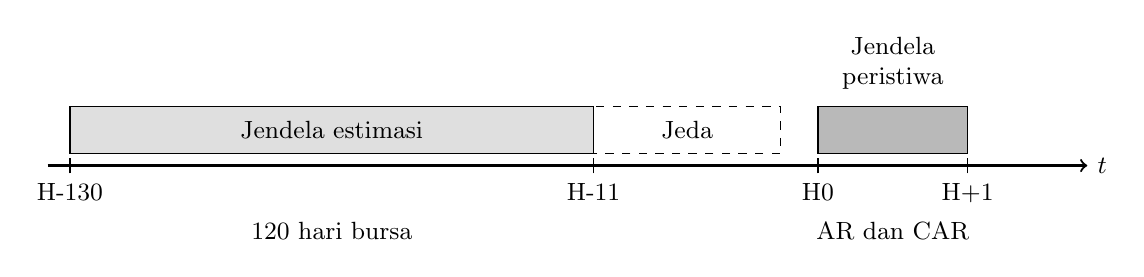
\begin{tikzpicture}[x=0.95cm, y=1cm, font=\small]
    % sumbu waktu
    \draw[->, thick] (-0.3,0) -- (13.6,0) node[right] {$t$};
    % jendela estimasi
    \fill[gray!25] (0,0.15) rectangle (7,0.75);
    \draw (0,0.15) rectangle (7,0.75);
    \node at (3.5,0.45) {Jendela estimasi};
    % jeda
    \draw[dashed] (7,0.15) rectangle (9.5,0.75);
    \node at (8.25,0.45) {Jeda};
    % jendela peristiwa
    \fill[gray!55] (10,0.15) rectangle (12,0.75);
    \draw (10,0.15) rectangle (12,0.75);
    \node[align=center] at (11,1.3) {Jendela\\peristiwa};
    % penanda hari
    \foreach \x/\lbl in {0/H-130, 7/H-11, 10/H0, 12/H+1} {
      \draw (\x,-0.1) -- (\x,0.1);
      \node[below] at (\x,-0.1) {\lbl};
    }
    \node[below, align=center] at (3.5,-0.6) {120 hari bursa};
    \node[below, align=center] at (11,-0.6) {AR dan CAR};
  \end{tikzpicture}
  \caption{Linimasa jendela estimasi dan jendela peristiwa yang digunakan dalam penelitian ini}
  \label{fig:linimasa-event-study}
\end{figure}

\subsection{\emph{Return}, \emph{Abnormal Return}, dan \emph{Cumulative Abnormal Return}}

\emph{Return} harian emiten $i$ pada hari $t$ dihitung dari perubahan harga penutupan terhadap hari bursa sebelumnya, seperti pada Persamaan~\ref{eq:return}. Harga $P_{i,t}$ yang digunakan merupakan harga yang telah disesuaikan terhadap \emph{stock split} dan dividen, sehingga peristiwa tersebut tidak terbaca sebagai lonjakan \emph{return}.
\begin{equation}
R_{i,t} = \frac{P_{i,t} - P_{i,t-1}}{P_{i,t-1}}
\label{eq:return}
\end{equation}
\eqcaption{\emph{Return} harian emiten}

\emph{Abnormal return} merupakan selisih antara \emph{return} aktual dan \emph{return} normal, yaitu \emph{return} yang diharapkan apabila peristiwa tidak terjadi \autocite{mackinlay1997}. Secara umum, \emph{abnormal return} dirumuskan pada Persamaan~\ref{eq:ar-umum}, dengan $X_t$ menyatakan informasi yang digunakan oleh model \emph{return} normal, misalnya \emph{return} pasar pada hari yang sama.
\begin{equation}
AR_{i,t} = R_{i,t} - E\left(R_{i,t} \mid X_t\right)
\label{eq:ar-umum}
\end{equation}
\eqcaption{\emph{Abnormal return}}

Reaksi harga terhadap suatu peristiwa tidak selalu selesai dalam satu hari. Untuk menangkap reaksi yang berlangsung selama beberapa hari, \emph{abnormal return} dijumlahkan sepanjang jendela peristiwa menjadi \emph{cumulative abnormal return} (CAR) seperti pada Persamaan~\ref{eq:car}. Target yang diprediksi dalam penelitian ini adalah $CAR_i[0,+1]$, yaitu jumlah \emph{abnormal return} pada H0 dan H+1. Pilihan ini sejalan dengan \textcite{mackinlay1997}, yang menyarankan jendela peristiwa setidaknya mencakup hari pengumuman dan hari setelahnya untuk menangkap pengumuman yang terjadi setelah pasar tutup. Pilihan ini juga mempertimbangkan kasus ARB yang membuat reaksi harga baru selesai pada hari berikutnya. Jendela yang mencakup H-1 tidak digunakan karena data H-1 juga menjadi bagian dari fitur model.
\begin{equation}
CAR_i[\tau_1, \tau_2] = \sum_{t=\tau_1}^{\tau_2} AR_{i,t}
\label{eq:car}
\end{equation}
\eqcaption{\emph{Cumulative abnormal return}}

Dalam \emph{event study} klasik, signifikansi \emph{abnormal return} diuji dengan membandingkannya terhadap simpangan baku residual model pada jendela estimasi \autocite{mackinlay1997}. Penelitian ini tidak menggunakan uji tersebut untuk menyimpulkan dampak satu jenis peristiwa, tetapi memakai gagasan yang sama untuk menentukan arah CAR aktual pada tahap evaluasi. Karena $CAR_i[0,+1]$ merupakan jumlah dua \emph{abnormal return} harian, variansnya merupakan jumlah varians kedua hari tersebut \autocite{mackinlay1997}. Apabila \emph{abnormal return} harian dianggap saling bebas dengan varians yang sama, simpangan baku CAR dua hari menjadi $\hat{\sigma}_{\varepsilon_i}\sqrt{2}$. Arah CAR aktual dikategorikan positif apabila nilainya lebih besar dari batas tersebut, negatif apabila lebih kecil dari batas negatifnya, dan netral untuk nilai di antaranya, seperti pada Persamaan~\ref{eq:zona-netral}. Dengan cara ini, zona netral menyesuaikan dengan tingkat volatilitas masing-masing emiten, sehingga emiten yang biasanya bergerak tajam memerlukan CAR yang lebih besar untuk dikategorikan positif atau negatif. Zona netral ini hanya digunakan untuk evaluasi, sedangkan model memprediksi besar CAR dan arah prediksinya dibaca dari tanda nilai yang diprediksi.
\begin{equation}
d_{i} =
\begin{cases}
\text{positif}, & CAR_i[0,+1] > \hat{\sigma}_{\varepsilon_i}\sqrt{2} \\
\text{negatif}, & CAR_i[0,+1] < -\hat{\sigma}_{\varepsilon_i}\sqrt{2} \\
\text{netral}, & \text{lainnya}
\end{cases}
\label{eq:zona-netral}
\end{equation}
\eqcaption{Arah CAR aktual dengan zona netral}

\section{Model \emph{Return} yang Diharapkan}
\label{sec:model-return}

Nilai \emph{abnormal return} sangat bergantung pada model yang digunakan untuk menghitung \emph{return} yang diharapkan. Semakin baik model menjelaskan pergerakan normal saham, semakin kecil varians \emph{abnormal return}, sehingga dampak suatu peristiwa lebih mudah dideteksi \autocite{mackinlay1997}. Subbab ini membahas beberapa model yang umum digunakan, mulai dari yang paling sederhana sampai model dua faktor yang digunakan dalam penelitian ini.

\subsection{Model Rata-Rata Konstan dan Model \emph{Market-Adjusted}}

Model rata-rata konstan mengasumsikan bahwa \emph{return} normal suatu saham sama dengan rata-rata \emph{return} saham tersebut pada jendela estimasi \autocite{mackinlay1997}. Model ini sederhana, tetapi tidak memperhitungkan kondisi pasar pada hari peristiwa. Akibatnya, ketika pasar sedang turun tajam, hampir seluruh saham akan terlihat memiliki \emph{abnormal return} negatif walaupun tidak ada peristiwa khusus. Model \emph{market-adjusted} mengatasi sebagian masalah tersebut dengan mengurangkan \emph{return} pasar secara langsung dari \emph{return} saham, seperti pada Persamaan~\ref{eq:market-adjusted}.
\begin{equation}
AR_{i,t} = R_{i,t} - R_{m,t}
\label{eq:market-adjusted}
\end{equation}
\eqcaption{\emph{Abnormal return} model \emph{market-adjusted}}

Model \emph{market-adjusted} tidak memerlukan jendela estimasi karena secara implisit mengasumsikan $\alpha = 0$ dan $\beta = 1$ untuk setiap saham. \textcite{brown1985} menunjukkan bahwa pada kasus tertentu, metode yang sederhana seperti ini juga dapat bekerja dengan baik. Model ini digunakan oleh \textcite{sudirman2026} dalam \emph{event study} di BEI dengan IHSG sebagai \emph{return} pasar. Kelemahannya, asumsi $\beta = 1$ tidak sesuai untuk saham yang bergerak jauh lebih tajam atau jauh lebih lambat daripada pasar. Selain itu, model ini sama sekali tidak memperhitungkan pengaruh sektor.

\subsection{\emph{Market Model}}

\emph{Market model} menghubungkan \emph{return} saham dengan \emph{return} pasar melalui regresi linear, seperti pada Persamaan~\ref{eq:market-model} \autocite{mackinlay1997}. Parameter $\alpha_i$ dan $\beta_i$ diestimasi menggunakan \emph{ordinary least squares} (OLS) pada jendela estimasi, kemudian digunakan untuk menghitung \emph{return} yang diharapkan pada jendela peristiwa. Nilai $\beta_i$ menunjukkan sensitivitas saham terhadap pergerakan pasar, sehingga saham yang biasanya bergerak lebih tajam daripada IHSG akan memiliki $\beta_i$ lebih besar dari satu.
\begin{equation}
R_{i,t} = \alpha_i + \beta_i R_{m,t} + \varepsilon_{i,t}, \quad E(\varepsilon_{i,t}) = 0, \quad \mathrm{Var}(\varepsilon_{i,t}) = \sigma^2_{\varepsilon_i}
\label{eq:market-model}
\end{equation}
\eqcaption{\emph{Market model}}

\textcite{brown1980} membandingkan beberapa metode pengukuran kinerja harga saham menggunakan data bulanan. Kajian serupa kemudian dilakukan oleh \textcite{brown1985} menggunakan data harian. Hasil kajian dengan data harian menunjukkan bahwa metode berbasis \emph{market model} yang sederhana sudah cukup tepat spesifikasinya dan memiliki kekuatan uji yang relatif baik pada berbagai kondisi. Temuan ini menjadikan \emph{market model} sebagai model standar dalam banyak \emph{event study}. Namun, \emph{market model} hanya menggunakan satu faktor, yaitu pasar. Apabila sebagian pergerakan saham sebenarnya berasal dari sektornya, bagian tersebut akan tertinggal di dalam residual dan ikut terhitung sebagai \emph{abnormal return}.

\subsection{Model Indeks Dua Faktor}

\textcite{mackinlay1997} menjelaskan bahwa model \emph{return} normal dapat diperluas menjadi model multifaktor dengan tujuan mengurangi varians \emph{abnormal return}, walaupun dalam banyak \emph{event study} manfaat tambahan faktor tersebut terbatas. Besarnya manfaat itu bergantung pada seberapa besar faktor tambahan dapat menjelaskan pergerakan saham yang tidak tertangkap oleh faktor pasar. Untuk faktor industri, bukti empiris diberikan oleh \textcite{xiang1993}. Penelitian tersebut membandingkan pilihan model pembangkit \emph{return} dalam \emph{event study} dan menemukan bahwa faktor industri menjelaskan rata-rata 6,7\% variasi residual \emph{market model} pada data harian dan 11,5\% pada data mingguan. Penelitian tersebut juga menyimpulkan bahwa apabila \emph{return} saham sebenarnya mengikuti model dua faktor, inferensi yang hanya didasarkan pada \emph{market model} menjadi tidak valid. Berdasarkan temuan tersebut, penelitian ini menggunakan model dua faktor seperti pada Persamaan~\ref{eq:dua-faktor}, dengan $R_{m,t}$ menyatakan \emph{return} IHSG dan $R_{s,t}$ menyatakan \emph{return} indeks sektoral IDX-IC tempat emiten diklasifikasikan.
\begin{equation}
R_{i,t} = \alpha_i + \beta_{1,i} R_{m,t} + \beta_{2,i} R_{s,t} + \varepsilon_{i,t}
\label{eq:dua-faktor}
\end{equation}
\eqcaption{Model indeks dua faktor}

Parameter $\alpha_i$, $\beta_{1,i}$, dan $\beta_{2,i}$ diestimasi dengan OLS pada jendela estimasi. \emph{Abnormal return} pada hari peristiwa kemudian dihitung sebagai selisih antara \emph{return} aktual dan \emph{return} yang diharapkan menurut parameter tersebut, seperti pada Persamaan~\ref{eq:ar-dua-faktor}. Simpangan baku residual $\hat{\sigma}_{\varepsilon_i}$ yang digunakan untuk menentukan zona netral pada Persamaan~\ref{eq:zona-netral} dihitung dari residual model pada jendela estimasi, seperti pada Persamaan~\ref{eq:sigma-residual}, dengan $L$ menyatakan jumlah hari bursa pada jendela estimasi.
\begin{equation}
AR_{i,t} = R_{i,t} - \left(\hat{\alpha}_i + \hat{\beta}_{1,i} R_{m,t} + \hat{\beta}_{2,i} R_{s,t}\right)
\label{eq:ar-dua-faktor}
\end{equation}
\eqcaption{\emph{Abnormal return} model dua faktor}
\begin{equation}
\hat{\sigma}_{\varepsilon_i} = \sqrt{\frac{1}{L - 3} \sum_{t \in \text{estimasi}} \hat{\varepsilon}_{i,t}^{\,2}}
\label{eq:sigma-residual}
\end{equation}
\eqcaption{Simpangan baku residual pada jendela estimasi}

Penggunaan bobot hasil regresi berbeda dengan sekadar mengurangkan \emph{return} IHSG dan \emph{return} sektor secara langsung. Indeks sektoral pada dasarnya juga ikut bergerak bersama IHSG, sehingga apabila keduanya dikurangkan secara penuh, pengaruh pasar akan terhitung dua kali. Sebagai ilustrasi, apabila IHSG turun 2\%, sektor turun 2\%, dan saham turun 3\%, pengurangan langsung menghasilkan $-3\% - (-2\%) - (-2\%) = +1\%$, seolah-olah saham tersebut mengungguli pasar padahal penurunannya paling dalam. Melalui regresi, besarnya keterikatan saham terhadap pasar dan sektor ditentukan dari data historis, sehingga masalah tersebut dapat dihindari. Perbandingan model-model yang telah dibahas dirangkum pada Tabel~\ref{tab:model-return}.

\begin{table}[t]
  \centering
  \caption{Perbandingan model \emph{return} yang diharapkan}
  \label{tab:model-return}
  \begin{tabularx}{\textwidth}{| p{2.6cm} | X | X |}
    \hline
    \textbf{Model} & \textbf{\emph{Return} yang diharapkan} & \textbf{Keterbatasan} \\
    \hline
    Rata-rata konstan & Rata-rata \emph{return} saham pada jendela estimasi & Tidak memperhitungkan kondisi pasar pada hari peristiwa \\
    \hline
    \emph{Market-adjusted} & \emph{Return} pasar pada hari yang sama & Mengasumsikan $\beta = 1$ dan tidak memperhitungkan sektor \\
    \hline
    \emph{Market model} & $\hat{\alpha}_i + \hat{\beta}_i R_{m,t}$ & Pergerakan sektor tertinggal di dalam \emph{abnormal return} \\
    \hline
    Dua faktor & $\hat{\alpha}_i + \hat{\beta}_{1,i} R_{m,t} + \hat{\beta}_{2,i} R_{s,t}$ & Estimasi $\beta$ dapat tidak stabil akibat kolinearitas, dan dapat menghapus dampak peristiwa berskala sektor \\
    \hline
  \end{tabularx}
\end{table}

Model dua faktor juga memiliki beberapa keterbatasan yang perlu diperhatikan. Pertama, \emph{return} IHSG dan \emph{return} indeks sektoral umumnya berkorelasi tinggi, terutama untuk sektor yang bobotnya besar di IHSG. Kolinearitas ini dapat membuat estimasi $\beta_{1,i}$ dan $\beta_{2,i}$ tidak stabil, walaupun nilai \emph{return} yang diharapkan secara keseluruhan masih dapat diestimasi. Salah satu cara untuk mengatasinya adalah meregresikan \emph{return} sektor terhadap \emph{return} IHSG terlebih dahulu, kemudian menggunakan residualnya sebagai faktor sektor, sehingga $\beta_{2,i}$ hanya menangkap pergerakan sektor di luar pergerakan pasar. Kedua, untuk peristiwa yang memengaruhi satu sektor secara keseluruhan, seperti perubahan regulasi pada suatu industri, koreksi sektor justru dapat menghapus dampak peristiwa tersebut karena seluruh emiten dalam sektor bergerak bersama. Oleh karena itu, untuk peristiwa berskala sektor, penelitian ini juga menghitung \emph{abnormal return} yang hanya dikoreksi oleh IHSG.

\section{Pemrosesan Teks Berita untuk Analisis Saham}
\label{sec:pemrosesan-teks}

\subsection{Sentimen dan Jenis Peristiwa}

Informasi dari teks berita dapat diekstraksi dalam berbagai bentuk. Bentuk yang paling banyak digunakan dalam penelitian keuangan adalah sentimen, yaitu ukuran nada positif atau negatif suatu teks. \textcite{kearney2014} merangkum berbagai metode dan model yang digunakan untuk mengukur sentimen tekstual di bidang keuangan, mulai dari pendekatan berbasis kamus kata sampai pendekatan berbasis \emph{machine learning}. Sentimen mudah diinterpretasikan dan dapat dihitung untuk hampir semua jenis teks. Namun, sentimen hanya menggambarkan nada berita, bukan peristiwa yang terjadi. Berita mengenai direktur yang ditetapkan sebagai tersangka korupsi dan berita mengenai laba yang turun sesuai ekspektasi analis sama-sama bernada negatif, tetapi keduanya merupakan peristiwa yang berbeda dan dapat diikuti reaksi harga yang berbeda pula.

Pendekatan lain adalah merepresentasikan berita berdasarkan peristiwa yang dikandungnya. \textcite{ding2015} mengekstraksi peristiwa dari teks berita dan merepresentasikannya sebagai vektor padat, kemudian menggunakan \emph{convolutional neural network} untuk memodelkan pengaruh jangka pendek dan jangka panjang peristiwa terhadap pergerakan harga. Model tersebut menghasilkan peningkatan sekitar 6\% dibandingkan metode pembanding pada prediksi indeks S\&P 500 dan saham individual. \textcite{zhou2021} memandang peristiwa korporasi sebagai penggerak pergerakan saham dan membangun detektor peristiwa dua tingkat, yaitu pada tingkat token dan tingkat artikel. Kedua penelitian tersebut menunjukkan bahwa jenis peristiwa dapat dijadikan representasi berita yang lebih spesifik dibandingkan sentimen. Pada penelitian ini, jenis peristiwa direpresentasikan sebagai label kategori yang dapat dibaca langsung, seperti hukum atau korupsi, laporan keuangan, dan pergantian direksi, sehingga kontribusinya terhadap prediksi dapat dijelaskan.

\subsection{Klasifikasi Berbasis Aturan dan Supervisi Lemah}

Cara paling sederhana untuk mengklasifikasikan jenis peristiwa adalah menggunakan aturan kata kunci. Misalnya, berita yang memuat kata ``tersangka'', ``KPK'', atau ``Kejagung'' diberi label hukum atau korupsi. Pendekatan ini mudah dibuat dan hasilnya transparan, tetapi tidak dapat menangani berita yang menggambarkan peristiwa yang sama dengan kata-kata berbeda. Selain itu, aturan kata kunci tidak memahami konteks, sehingga kata yang sama dapat muncul pada berita dengan peristiwa yang berbeda.

Walaupun kurang akurat jika digunakan sebagai \emph{classifier} akhir, aturan kata kunci dapat dimanfaatkan untuk mempercepat penyusunan data latih. \textcite{ratner2017} memperkenalkan Snorkel, yaitu sistem yang memungkinkan pengguna menulis fungsi pelabelan berupa aturan atau heuristik untuk menghasilkan label data latih tanpa melabeli setiap data secara manual. Pendekatan ini dikenal sebagai supervisi lemah karena label yang dihasilkan masih mengandung kesalahan. Pada penelitian ini, gagasan tersebut digunakan dalam bentuk yang lebih sederhana, yaitu aturan kata kunci menghasilkan pra-label yang kemudian diperiksa dan dikoreksi secara manual.

\subsection{TF-IDF dengan Logistic Regression dan SVM}

Pendekatan klasik untuk klasifikasi teks adalah merepresentasikan dokumen sebagai vektor bobot kata, kemudian melatih \emph{classifier} linear di atas vektor tersebut. Salah satu skema pembobotan yang paling umum adalah TF-IDF (\emph{term frequency-inverse document frequency}). Bobot ini memberikan nilai tinggi kepada kata yang sering muncul pada suatu dokumen tetapi jarang muncul pada dokumen lain. Gagasan bahwa kata yang muncul di banyak dokumen memiliki daya pembeda yang lebih rendah diperkenalkan oleh \textcite{sparckjones1972}. Bobot TF-IDF kata $w$ pada dokumen $d$ dihitung seperti pada Persamaan~\ref{eq:tfidf}, dengan $\mathrm{tf}(w,d)$ menyatakan frekuensi kata $w$ pada dokumen $d$, $N$ menyatakan jumlah dokumen, dan $\mathrm{df}(w)$ menyatakan jumlah dokumen yang memuat kata $w$.
\begin{equation}
\text{tf-idf}(w,d) = \mathrm{tf}(w,d) \cdot \log \frac{N}{\mathrm{df}(w)}
\label{eq:tfidf}
\end{equation}
\eqcaption{Bobot TF-IDF}

Vektor TF-IDF umumnya berdimensi tinggi dan bersifat jarang. \textcite{joachims1998} menunjukkan bahwa \emph{support vector machine} (SVM) cocok untuk klasifikasi teks karena mampu menangani ruang fitur berdimensi tinggi dengan banyak fitur yang relevan. \emph{Logistic regression} juga sering digunakan karena sederhana dan menghasilkan probabilitas kelas. Kelemahan pendekatan ini adalah setiap kata diperlakukan secara terpisah, sehingga urutan kata dan konteks kalimat tidak tertangkap. Meskipun demikian, kombinasi TF-IDF dengan SVM atau \emph{logistic regression} tetap menjadi pendekatan yang kuat dan murah secara komputasi untuk klasifikasi teks.

\subsection{Transformer, BERT, dan IndoBERT}

Transformer merupakan arsitektur jaringan saraf yang sepenuhnya menggunakan mekanisme \emph{attention} untuk memodelkan hubungan antartoken dalam suatu urutan \autocite{vaswani2017}. Mekanisme \emph{self-attention} memungkinkan representasi setiap token dihitung dengan mempertimbangkan seluruh token lain dalam kalimat. Berdasarkan arsitektur tersebut, \textcite{devlin2019} memperkenalkan BERT (\emph{Bidirectional Encoder Representations from Transformers}), yaitu model \emph{encoder} yang dilatih awal pada korpus teks besar menggunakan tugas \emph{masked language modeling} dan \emph{next sentence prediction}. Representasi yang dihasilkan bersifat dua arah, karena setiap token dipahami berdasarkan konteks di sebelah kiri dan kanannya. Setelah dilatih awal, BERT dapat disesuaikan untuk tugas tertentu melalui \emph{fine-tuning}, yaitu dengan menambahkan lapisan klasifikasi dan melatih ulang model menggunakan data berlabel dalam jumlah yang relatif kecil.

Untuk bahasa Indonesia, \textcite{wilie2020} merilis IndoNLU, yaitu kumpulan dua belas tugas pemahaman bahasa Indonesia beserta model IndoBERT yang dilatih awal pada korpus Indo4B. Korpus tersebut dikumpulkan dari sumber publik seperti media sosial, blog, berita, dan situs web. Salah satu varian yang dirilis adalah \texttt{indobenchmark/indobert-base-p1}. Pada waktu yang hampir bersamaan, \textcite{koto2020} juga merilis model IndoBERT lain beserta tolok ukur IndoLEM, sehingga nama IndoBERT dalam literatur dapat merujuk pada dua model yang berbeda. Untuk domain keuangan, \textcite{maharani2023} melakukan \emph{post-training} model bahasa pada korpus keuangan Indonesia dan menyusun dataset analisis sentimen serta klasifikasi topik keuangan berbahasa Indonesia. Penelitian tersebut menemukan bahwa \emph{post-training} pada domain keuangan meningkatkan kinerja model ketika di-\emph{fine-tune} untuk tugas pada domain yang sama.

Perlu dibedakan bahwa IndoBERT merupakan model \emph{encoder} yang di-\emph{fine-tune} untuk tugas klasifikasi, bukan model bahasa generatif. Model ini menghasilkan probabilitas untuk setiap kelas yang telah ditentukan dan tidak menghasilkan teks baru. Dengan bobot model yang tetap setelah pelatihan, keluaran IndoBERT untuk masukan yang sama akan selalu sama. Sifat ini mendukung kebutuhan penelitian ini akan \emph{pipeline} yang dapat direproduksi.

\subsection{Anotasi dan Kesepakatan Antaranotator}

Model klasifikasi jenis peristiwa memerlukan data berlabel, dan kualitas label perlu diukur sebelum data digunakan untuk evaluasi. Apabila dua anotator melabeli data yang sama, kesepakatan antara keduanya dapat diukur dengan Cohen's kappa \autocite{cohen1960}. Berbeda dengan persentase kesepakatan biasa, kappa mengoreksi kesepakatan yang dapat terjadi secara kebetulan, seperti pada Persamaan~\ref{eq:kappa}. Pada persamaan tersebut, $p_o$ menyatakan proporsi data yang labelnya sama di antara kedua anotator, sedangkan $p_e$ menyatakan proporsi kesepakatan yang diharapkan secara kebetulan berdasarkan distribusi label masing-masing anotator.
\begin{equation}
\kappa = \frac{p_o - p_e}{1 - p_e}
\label{eq:kappa}
\end{equation}
\eqcaption{Cohen's kappa}

\textcite{landis1977} mengusulkan interpretasi nilai kappa ke dalam beberapa tingkat. Nilai 0,41 sampai 0,60 dikategorikan sebagai kesepakatan sedang (\emph{moderate}), nilai 0,61 sampai 0,80 sebagai kesepakatan substansial (\emph{substantial}), dan nilai di atas 0,80 sebagai kesepakatan hampir sempurna (\emph{almost perfect}). Berdasarkan interpretasi tersebut, target kappa sekurang-kurangnya 0,6 pada penelitian ini berada pada batas antara kesepakatan sedang dan substansial. Nilai kappa yang lebih rendah dari target menunjukkan bahwa definisi kategori dalam pedoman anotasi belum cukup jelas, sehingga pedoman perlu diperbaiki sebelum pelabelan dilanjutkan.

\section{Model Regresi untuk Prediksi CAR}
\label{sec:model-regresi}

Prediksi besar $CAR[0,+1]$ merupakan masalah regresi, yaitu memetakan fitur berita dan kondisi pasar menjadi satu nilai numerik dalam satuan persen. Penelitian ini membandingkan empat model regresi, yaitu Linear Regression, Random Forest, XGBoost, dan LightGBM. Arah CAR tidak diprediksi dengan model klasifikasi terpisah, melainkan dibaca dari tanda nilai yang diprediksi. Pendekatan ini serupa dengan \textcite{amelzadeh2020}, yang melatih model dalam bentuk regresi untuk memprediksi \emph{abnormal return} di sekitar pengumuman laba, kemudian menilai ketepatan tanda prediksinya. Subbab ini membahas keempat model tersebut beserta alasan penggunaan model berbasis pohon untuk data tabular.

\subsection{Linear Regression}

Linear Regression memodelkan target sebagai kombinasi linear dari fitur, seperti pada Persamaan~\ref{eq:linreg}, dengan $\hat{y}_i$ menyatakan prediksi untuk data ke-$i$, $x_{i,j}$ menyatakan nilai fitur ke-$j$, dan $w_j$ menyatakan bobot fitur. Bobot diestimasi dengan meminimalkan jumlah kuadrat selisih antara target aktual dan prediksi, sama seperti OLS yang digunakan pada model \emph{return} yang diharapkan. Kelebihan model ini adalah sederhana dan mudah diinterpretasikan, karena setiap bobot menunjukkan perubahan prediksi untuk setiap kenaikan satu satuan fitur. Kelemahannya, model ini mengasumsikan hubungan yang linear dan tidak menangkap interaksi antarfitur kecuali interaksi tersebut ditambahkan secara eksplisit. Model linear seperti OLS dan Lasso banyak digunakan sebagai pembanding dalam penelitian prediksi \emph{return} \autocite{gu2020,amelzadeh2020}, sehingga dalam penelitian ini Linear Regression berperan sebagai model pembanding yang paling sederhana.
\begin{equation}
\hat{y}_i = w_0 + \sum_{j=1}^{M} w_j x_{i,j}
\label{eq:linreg}
\end{equation}
\eqcaption{Linear Regression}

\subsection{Random Forest}

Random Forest merupakan kumpulan pohon keputusan yang masing-masing dilatih pada sampel \emph{bootstrap} dari data latih, dengan pemilihan subhimpunan fitur secara acak pada setiap pemisahan simpul \autocite{breiman2001}. Untuk regresi, prediksi akhir merupakan rata-rata keluaran seluruh pohon, seperti pada Persamaan~\ref{eq:rf}, dengan $B$ menyatakan jumlah pohon dan $T_b$ menyatakan pohon ke-$b$. Keacakan pada sampel dan fitur membuat setiap pohon berbeda, sehingga rata-ratanya lebih stabil dibandingkan satu pohon keputusan. Pada prediksi \emph{abnormal return} di sekitar pengumuman laba, \textcite{amelzadeh2020} menemukan bahwa Random Forest dan \emph{recurrent neural network} mengungguli \emph{deep neural network} serta model linear seperti OLS dan Lasso. \textcite{schnaubelt2020} juga menemukan bahwa Random Forest menghasilkan \emph{abnormal return} portofolio yang lebih tinggi dibandingkan tiga model pembanding pada lebih dari 45.000 pengumuman laba.
\begin{equation}
\hat{y}_i = \frac{1}{B} \sum_{b=1}^{B} T_b(\mathbf{x}_i)
\label{eq:rf}
\end{equation}
\eqcaption{Prediksi Random Forest}

\subsection{\emph{Gradient Boosting} dan XGBoost}

Berbeda dengan Random Forest yang membangun pohon secara paralel, \emph{gradient boosting} membangun model secara bertahap dengan menambahkan model lemah satu per satu. \textcite{friedman2001} merumuskan metode ini sebagai optimasi numerik dalam ruang fungsi, yaitu setiap model baru ditambahkan ke arah gradien negatif dari fungsi kerugian. Dalam praktiknya, model lemah yang digunakan umumnya berupa pohon keputusan, sehingga hasil akhirnya merupakan jumlah dari banyak pohon. Setiap pohon baru berfokus memperbaiki kesalahan yang masih tersisa dari pohon-pohon sebelumnya.

XGBoost merupakan implementasi \emph{tree boosting} yang dirancang agar dapat diskalakan dan efisien \autocite{chen2016}. Prediksi XGBoost untuk data ke-$i$ merupakan jumlah keluaran $K$ pohon, seperti pada Persamaan~\ref{eq:xgb-prediksi}. Model dilatih dengan meminimalkan fungsi objektif yang terdiri dari fungsi kerugian $l$ dan suku regularisasi $\Omega$, seperti pada Persamaan~\ref{eq:xgb-objektif}. Pada suku regularisasi, $T$ menyatakan jumlah daun pada pohon, $w$ menyatakan bobot daun, sedangkan $\gamma$ dan $\lambda$ merupakan parameter yang mengatur besarnya penalti kompleksitas pohon.
\begin{equation}
\hat{y}_i = \sum_{k=1}^{K} f_k(\mathbf{x}_i)
\label{eq:xgb-prediksi}
\end{equation}
\eqcaption{Prediksi XGBoost}
\begin{equation}
\mathcal{L} = \sum_{i} l\left(y_i, \hat{y}_i\right) + \sum_{k} \Omega(f_k), \quad \Omega(f) = \gamma T + \frac{1}{2} \lambda \lVert w \rVert^2
\label{eq:xgb-objektif}
\end{equation}
\eqcaption{Fungsi objektif XGBoost}

Selain regularisasi, \textcite{chen2016} juga mengusulkan algoritma yang memperhitungkan data jarang dan metode \emph{weighted quantile sketch} untuk pencarian titik pemisah secara aproksimatif. XGBoost dapat digunakan untuk klasifikasi maupun regresi dengan mengganti fungsi kerugiannya. Tinjauan sistematis \textcite{cerneviciene2024} mencatat bahwa XGBoost termasuk tiga model \emph{black-box} yang paling sering dijelaskan dengan metode XAI dalam penelitian keuangan, bersama \emph{artificial neural network} dan Random Forest.

\subsection{LightGBM}

LightGBM merupakan implementasi \emph{gradient boosting decision tree} yang dirancang untuk mempercepat pelatihan pada data dengan jumlah fitur dan jumlah data yang besar \autocite{ke2017}. \textcite{ke2017} mengusulkan dua teknik utama. Teknik pertama adalah \emph{Gradient-based One-Side Sampling} (GOSS), yaitu mempertahankan data dengan gradien besar dan mengambil sampel acak dari data dengan gradien kecil, karena data dengan gradien besar lebih berpengaruh terhadap perhitungan perolehan informasi. Teknik kedua adalah \emph{Exclusive Feature Bundling} (EFB), yaitu menggabungkan fitur-fitur yang jarang bernilai bukan nol secara bersamaan untuk mengurangi jumlah fitur. Dengan kedua teknik tersebut, LightGBM dapat mempercepat pelatihan \emph{gradient boosting} konvensional hingga lebih dari 20 kali dengan akurasi yang hampir sama. Kecepatan ini relevan bagi penelitian ini karena penyetelan \emph{hyperparameter} dilakukan untuk setiap model.

LightGBM juga telah digunakan dalam penelitian prediksi saham. \textcite{pagliaro2026} menggunakan LightGBM untuk memprediksi arah \emph{return} sepuluh hari ke depan pada 51 saham konstituen NASDAQ-100 periode 2015 sampai 2026 dan menemukan bahwa model tersebut mengungguli empat model pembanding. Penelitian tersebut memilih LightGBM karena keunggulannya pada data keuangan tabular dan kesesuaiannya dengan TreeSHAP, kemudian menggunakan SHAP untuk menjelaskan kontribusi fitur. \textcite{tian2022} membandingkan model hibrida LSTM dengan LightGBM dan LSTM dengan XGBoost untuk memprediksi naik turunnya harga, dan menemukan bahwa versi yang menggunakan LightGBM memberikan hasil terbaik. Pada pasar negara berkembang, \textcite{guennioui2024} menggunakan LightGBM untuk memprediksi harga saham di pasar Maroko selama periode volatilitas tinggi, termasuk analisis per sektor. Ketiga penelitian tersebut memprediksi harga atau arah \emph{return} mentah, sehingga penggunaan LightGBM untuk memprediksi \emph{abnormal return} yang dikoreksi pasar dan sektor masih perlu diuji.

\subsection{Model Berbasis Pohon pada Data Tabular}

Data yang digunakan dalam penelitian ini berbentuk tabular, yaitu satu baris untuk setiap pasangan berita dan emiten dengan fitur kategorikal dan numerik. \textcite{grinsztajn2022} menguji model berbasis pohon dan model \emph{deep learning} pada 45 dataset tabular dan menemukan bahwa model berbasis pohon tetap menjadi yang terbaik pada data berukuran sedang, sekitar 10.000 sampel. \textcite{shwartzziv2022} juga menemukan bahwa XGBoost umumnya mengungguli model \emph{deep learning} yang dirancang khusus untuk data tabular. Pada prediksi \emph{return} saham, \textcite{gu2020} menemukan bahwa model berbasis pohon dan \emph{neural network} memberikan hasil terbaik karena mampu menangkap interaksi nonlinear antarprediktor yang tidak tertangkap oleh model linear. Temuan-temuan tersebut menjadi dasar pemilihan tiga model berbasis pohon dalam penelitian ini, dengan Linear Regression sebagai pembanding. Model berbasis pohon juga memungkinkan nilai SHAP dihitung secara tepat dan efisien, seperti yang dibahas pada subbab berikutnya.

\section{Metode \emph{Explainable AI}}
\label{sec:xai}

Model seperti Random Forest, XGBoost, dan LightGBM dapat menghasilkan prediksi yang akurat, tetapi alasan di balik setiap prediksinya tidak dapat dibaca secara langsung. Metode \emph{explainable AI} (XAI) digunakan untuk menjelaskan kontribusi fitur terhadap prediksi tersebut. Metode XAI dapat dibedakan berdasarkan cakupannya, yaitu penjelasan lokal untuk satu prediksi dan penjelasan global untuk perilaku model secara keseluruhan, serta berdasarkan ketergantungannya pada jenis model, yaitu metode khusus untuk model tertentu dan metode yang dapat diterapkan pada model apa pun (\emph{model-agnostic}). \textcite{arsenault2025} juga menekankan pentingnya membedakan \emph{explainability} dan \emph{interpretability} dalam penerapan XAI untuk prediksi runtun waktu keuangan. Penelitian ini membandingkan tiga metode XAI yang mewakili pendekatan berbeda, yaitu SHAP, LIME, dan \emph{permutation importance}.

\subsection{SHAP}

SHAP (\emph{SHapley Additive exPlanations}) merupakan kerangka yang memberikan nilai kepentingan setiap fitur untuk suatu prediksi tertentu \autocite{lundberg2017}. SHAP termasuk dalam kelompok metode atribusi fitur aditif, yaitu metode yang menjelaskan prediksi sebagai jumlah dari nilai dasar dan kontribusi setiap fitur, seperti pada Persamaan~\ref{eq:shap-aditif}. Pada persamaan tersebut, $\phi_0$ merupakan nilai dasar yang setara dengan rata-rata prediksi model, $M$ merupakan jumlah fitur, $z'_j$ menyatakan ada atau tidaknya fitur $j$, dan $\phi_j$ merupakan kontribusi fitur $j$.
\begin{equation}
g(z') = \phi_0 + \sum_{j=1}^{M} \phi_j z'_j
\label{eq:shap-aditif}
\end{equation}
\eqcaption{Model penjelasan aditif SHAP}

Nilai $\phi_j$ dihitung berdasarkan nilai Shapley dari teori permainan kooperatif \autocite{shapley1953}. Dalam konteks ini, setiap fitur diperlakukan sebagai pemain, dan prediksi model diperlakukan sebagai hasil yang dibagikan kepada para pemain. Nilai Shapley fitur $j$ merupakan rata-rata kontribusi marginal fitur tersebut terhadap seluruh kemungkinan subhimpunan fitur lain, seperti pada Persamaan~\ref{eq:shapley}, dengan $F$ menyatakan himpunan seluruh fitur dan $f_x(S)$ menyatakan prediksi model ketika hanya fitur dalam subhimpunan $S$ yang diketahui.
\begin{equation}
\phi_j = \sum_{S \subseteq F \setminus \{j\}} \frac{|S|!\,\left(|F| - |S| - 1\right)!}{|F|!} \left[ f_x\left(S \cup \{j\}\right) - f_x(S) \right]
\label{eq:shapley}
\end{equation}
\eqcaption{Nilai Shapley}

\textcite{lundberg2017} menunjukkan bahwa dalam kelompok metode atribusi aditif terdapat satu solusi unik yang memenuhi sifat akurasi lokal, \emph{missingness}, dan konsistensi, dan solusi tersebut adalah nilai Shapley. Akurasi lokal berarti jumlah nilai dasar dan seluruh kontribusi fitur sama dengan prediksi model untuk data tersebut. Perhitungan Persamaan~\ref{eq:shapley} secara langsung memerlukan evaluasi pada seluruh subhimpunan fitur, sehingga waktu komputasinya tumbuh secara eksponensial terhadap jumlah fitur. \textcite{lundberg2020} kemudian mengusulkan TreeSHAP, yaitu algoritma yang menghitung nilai SHAP secara tepat untuk model berbasis pohon dalam waktu polinomial, serta menunjukkan bahwa penjelasan lokal dapat digabungkan untuk memahami perilaku model secara global. Karena target penelitian ini adalah besar CAR, nilai SHAP dinyatakan dalam satuan yang sama dengan target, yaitu persen CAR, sehingga kontribusi setiap fitur dapat dibaca langsung.

\subsection{LIME}

LIME (\emph{Local Interpretable Model-agnostic Explanations}) menjelaskan satu prediksi dengan membangun model sederhana yang dapat diinterpretasikan di sekitar data yang dijelaskan \autocite{ribeiro2016}. LIME membuat sejumlah sampel tiruan dengan mengubah nilai fitur di sekitar data tersebut, meminta prediksi model untuk setiap sampel, kemudian melatih model sederhana seperti regresi linear dengan bobot yang lebih besar untuk sampel yang lebih dekat dengan data asli. Secara formal, penjelasan $\xi(x)$ diperoleh dari Persamaan~\ref{eq:lime}, dengan $f$ menyatakan model yang dijelaskan, $g$ menyatakan model sederhana dari kelompok model $G$, $\pi_x$ menyatakan ukuran kedekatan terhadap data $x$, $\mathcal{L}$ menyatakan seberapa jauh $g$ menyimpang dari $f$ di sekitar $x$, dan $\Omega(g)$ menyatakan kompleksitas model sederhana tersebut.
\begin{equation}
\xi(x) = \operatorname*{arg\,min}_{g \in G} \; \mathcal{L}\left(f, g, \pi_x\right) + \Omega(g)
\label{eq:lime}
\end{equation}
\eqcaption{Objektif LIME}

Karena hanya membutuhkan masukan dan keluaran model, LIME dapat diterapkan pada model apa pun. \textcite{gite2021} menggunakan LIME untuk menjelaskan prediksi harga saham berbasis LSTM yang memanfaatkan sentimen berita. Kelemahannya, sampel tiruan dibuat secara acak, sehingga penjelasan untuk data yang sama dapat berbeda apabila dijalankan ulang \autocite{zhang2019}. Selain itu, \textcite{alvarezmelis2018} menunjukkan bahwa metode populer seperti LIME dan SHAP dapat menghasilkan penjelasan yang berubah cukup besar akibat perubahan kecil pada input, dan metode yang berbasis perturbasi cenderung lebih rentan terhadap masalah ini.

\subsection{\emph{Permutation Importance}}

\emph{Permutation importance} mengukur kepentingan suatu fitur dari seberapa besar kinerja model menurun ketika nilai fitur tersebut diacak. Gagasan ini diperkenalkan oleh \textcite{breiman2001} pada Random Forest dan dikembangkan oleh \textcite{fisher2019} menjadi ukuran yang dapat diterapkan pada model apa pun. Kepentingan fitur $j$ dihitung seperti pada Persamaan~\ref{eq:perm-importance}, dengan $e(f; X)$ menyatakan kesalahan model, misalnya MAE, pada data asli dan $e(f; X^{(j)})$ menyatakan kesalahan model setelah nilai fitur $j$ diacak antarbaris. Semakin besar kenaikan kesalahan, semakin penting fitur tersebut bagi model.
\begin{equation}
PI_j = e\left(f; X^{(j)}\right) - e\left(f; X\right)
\label{eq:perm-importance}
\end{equation}
\eqcaption{\emph{Permutation importance}}

Berbeda dengan SHAP dan LIME, \emph{permutation importance} hanya menghasilkan penjelasan global dan tidak dapat menjelaskan satu prediksi tertentu. Kelebihannya, metode ini sederhana, tidak bergantung pada struktur model, dan langsung terkait dengan metrik kinerja yang digunakan.

\subsection{Kriteria Perbandingan Metode XAI}

Perbedaan cara kerja ketiga metode tersebut dirangkum pada Tabel~\ref{tab:metode-xai}. Karena setiap metode dapat menghasilkan penjelasan yang berbeda untuk model yang sama, perbandingannya memerlukan kriteria yang jelas. Kriteria pertama adalah kestabilan, yaitu apakah penjelasan untuk data yang sama tetap serupa ketika metode dijalankan berulang \autocite{zhang2019} atau ketika input diubah sedikit \autocite{alvarezmelis2018}. Kriteria kedua adalah kesepakatan antarmetode, yaitu apakah ketiga metode menunjukkan urutan fitur penting yang serupa pada tingkat global, dengan penjelasan lokal SHAP dan LIME dirata-ratakan terlebih dahulu. Kriteria ketiga adalah waktu komputasi yang dibutuhkan setiap metode. Tinjauan \textcite{cerneviciene2024} juga mencatat bahwa banyak penelitian keuangan menggabungkan beberapa metode XAI dalam satu kerangka penjelasan, sehingga perbandingan antarmetode menjadi relevan.

\begin{table}[t]
  \centering
  \caption{Perbandingan karakteristik metode XAI yang digunakan}
  \label{tab:metode-xai}
  \begin{tabularx}{\textwidth}{| >{\raggedright\arraybackslash}p{3.0cm} | >{\raggedright\arraybackslash}X | >{\raggedright\arraybackslash}X | >{\raggedright\arraybackslash}X |}
    \hline
    \textbf{Aspek} & \textbf{SHAP} & \textbf{LIME} & \textbf{\emph{Permutation importance}} \\
    \hline
    Cakupan & Lokal dan global & Lokal & Global \\
    \hline
    Ketergantungan model & TreeSHAP khusus model pohon, varian lain \emph{model-agnostic} & \emph{Model-agnostic} & \emph{Model-agnostic} \\
    \hline
    Unsur acak & Tidak ada pada TreeSHAP & Sampel tiruan acak & Pengacakan nilai fitur \\
    \hline
    Satuan penjelasan & Satuan target (persen CAR) & Bobot model sederhana & Kenaikan kesalahan \\
    \hline
  \end{tabularx}
\end{table}

\section{Metrik Evaluasi dan Uji Signifikansi}
\label{sec:metrik-evaluasi}

\subsection{Metrik Regresi}

Kinerja prediksi besar CAR diukur menggunakan \emph{mean absolute error} (MAE) dan \emph{root mean squared error} (RMSE), seperti pada Persamaan~\ref{eq:mae} dan Persamaan~\ref{eq:rmse}, dengan $n$ menyatakan jumlah data uji. MAE menyatakan rata-rata besar kesalahan dalam satuan yang sama dengan target, sehingga mudah diinterpretasikan sebagai rata-rata selisih persen antara CAR prediksi dan CAR aktual. \textcite{willmott2005} berpendapat bahwa MAE merupakan ukuran rata-rata kesalahan yang lebih alami dibandingkan RMSE, karena RMSE juga dipengaruhi oleh sebaran besarnya kesalahan. Meskipun demikian, RMSE tetap dilaporkan karena memberikan penalti lebih besar terhadap kesalahan yang besar. Hal ini relevan karena CAR dapat memiliki nilai ekstrem, misalnya pada berita kasus hukum besar.
\begin{equation}
\mathrm{MAE} = \frac{1}{n} \sum_{i=1}^{n} \left| y_i - \hat{y}_i \right|
\label{eq:mae}
\end{equation}
\eqcaption{\emph{Mean absolute error}}
\begin{equation}
\mathrm{RMSE} = \sqrt{\frac{1}{n} \sum_{i=1}^{n} \left( y_i - \hat{y}_i \right)^2}
\label{eq:rmse}
\end{equation}
\eqcaption{\emph{Root mean squared error}}

\subsection{Ketepatan Arah dengan Zona Netral}

Arah prediksi dibaca dari tanda nilai CAR yang diprediksi, sedangkan arah aktual ditentukan dari CAR aktual dengan zona netral pada Persamaan~\ref{eq:zona-netral}. Sampel dengan CAR aktual di dalam zona netral tidak menunjukkan pergerakan yang berarti, sehingga tidak tepat apabila model dinilai benar atau salah dalam menebak arahnya. Karena itu, ketepatan arah dihitung hanya pada sampel yang CAR aktualnya berada di luar zona netral, seperti pada Persamaan~\ref{eq:ketepatan-arah}, dengan $S$ menyatakan himpunan sampel tersebut dan $\mathbb{1}[\cdot]$ bernilai satu apabila kondisi di dalamnya terpenuhi. Gagasan ini serupa dengan \textcite{amelzadeh2020}, yang menilai persentase ketepatan tanda prediksi untuk reaksi pasar dengan berbagai ambang besar reaksi. Ketepatan tanda pada seluruh sampel tanpa zona netral juga dilaporkan sebagai pelengkap.
\begin{equation}
DA = \frac{1}{|S|} \sum_{i \in S} \mathbb{1}\left[ \operatorname{sign}(\hat{y}_i) = \operatorname{sign}(y_i) \right], \qquad S = \left\{ i : |y_i| > \hat{\sigma}_{\varepsilon_i} \sqrt{2} \right\}
\label{eq:ketepatan-arah}
\end{equation}
\eqcaption{Ketepatan arah dengan zona netral}

\subsection{Metrik Klasifikasi Jenis Peristiwa}

Kualitas \emph{classifier} jenis peristiwa yang digunakan untuk menghasilkan fitur diukur pada \emph{test set} emas menggunakan accuracy dan F1-macro. Accuracy menyatakan proporsi prediksi yang benar, tetapi nilainya dapat menyesatkan ketika distribusi kelas tidak seimbang, misalnya ketika kategori kebijakan pemerintah jauh lebih jarang muncul dibandingkan laporan keuangan. Untuk itu, digunakan F1-macro, yaitu rata-rata F1 dari setiap kelas tanpa pembobotan berdasarkan jumlah data \autocite{sokolova2009}. F1 untuk kelas $c$ merupakan rata-rata harmonik dari \emph{precision} $P_c$ dan \emph{recall} $R_c$, seperti pada Persamaan~\ref{eq:f1-macro}, dengan $C$ menyatakan jumlah kelas.
\begin{equation}
F1_c = \frac{2 P_c R_c}{P_c + R_c}, \qquad \text{F1-macro} = \frac{1}{C} \sum_{c=1}^{C} F1_c
\label{eq:f1-macro}
\end{equation}
\eqcaption{F1 per kelas dan F1-macro}

\subsection{Uji Signifikansi Selisih Kinerja}

Selisih metrik antara dua model pada satu data uji belum tentu menunjukkan perbedaan yang nyata, karena selisih tersebut dapat muncul akibat variasi sampel. Untuk membandingkan ketepatan arah dua model pada data uji yang sama, dapat digunakan uji McNemar \autocite{mcnemar1947}. \textcite{dietterich1998} membandingkan beberapa uji statistik untuk membandingkan algoritma pembelajaran dan merekomendasikan uji McNemar untuk kondisi ketika model hanya dapat dilatih dan diuji satu kali. Statistik uji McNemar dengan koreksi kontinuitas ditunjukkan pada Persamaan~\ref{eq:mcnemar}, dengan $n_{01}$ menyatakan jumlah sampel yang arahnya salah ditebak oleh model pertama tetapi benar oleh model kedua, dan $n_{10}$ menyatakan kebalikannya. Statistik ini mengikuti distribusi $\chi^2$ dengan satu derajat kebebasan.
\begin{equation}
\chi^2 = \frac{\left( \left| n_{01} - n_{10} \right| - 1 \right)^2}{n_{01} + n_{10}}
\label{eq:mcnemar}
\end{equation}
\eqcaption{Statistik uji McNemar}

Uji McNemar hanya berlaku untuk perbandingan benar atau salah, sehingga tidak dapat digunakan untuk metrik seperti MAE dan RMSE. Untuk metrik tersebut, digunakan metode \emph{bootstrap} \autocite{efron1979}. Pada metode ini, data uji diambil ulang secara acak dengan pengembalian sebanyak ratusan sampai ribuan kali, kemudian selisih metrik kedua model dihitung pada setiap sampel ulang. Distribusi selisih yang diperoleh digunakan untuk menyusun selang kepercayaan. Apabila selang kepercayaan tersebut tidak memuat nol, selisih kinerja kedua model dapat dianggap signifikan pada tingkat kepercayaan yang digunakan.

\section{Penelitian Terkait}
\label{sec:penelitian-terkait}

Penelitian terkait pada subbab ini dikelompokkan menjadi lima, yaitu penelitian berbasis berita di Indonesia, \emph{event study} di BEI, penelitian yang menghubungkan peristiwa dari teks dengan \emph{abnormal return}, penelitian yang membandingkan model untuk prediksi \emph{return}, serta penelitian yang menggunakan \emph{explainable AI} untuk prediksi saham. Pengelompokan ini digunakan untuk melihat komponen apa saja yang sudah dikerjakan oleh penelitian sebelumnya dan komponen apa yang belum.

\subsection{Penelitian Berbasis Berita di Indonesia}

\textcite{attar2024} menggunakan IndoBERT untuk mengklasifikasikan sentimen 2.857 berita saham dan memperoleh akurasi 0,78. Hasil klasifikasi tersebut kemudian dikorelasikan dengan pergerakan harga per sektor, dengan korelasi Pearson tertinggi sebesar 0,389 pada sektor \emph{basic materials}. \textcite{alamsyah2025} menganalisis 192.582 berita keuangan Indonesia periode 2018 sampai 2023, mendeteksi perusahaan yang disebutkan dalam berita, dan menyusun jaringan kemunculan bersama antarperusahaan. Penelitian tersebut menemukan bahwa korelasi sentimen dengan harga meningkat dari 0,26 pada tingkat perusahaan menjadi 0,30 pada tingkat industri dan 0,43 pada klaster perusahaan yang sering muncul bersama dalam berita. Temuan ini menunjukkan bahwa pengelompokan berdasarkan industri dan kemunculan bersama dapat memperjelas hubungan antara berita dan harga.

\textcite{kusuma2026} menggabungkan sentimen IndoBERT dari 9.819 berita CNBC Indonesia dengan data harga untuk mengklasifikasikan tren harga lima emiten LQ45 menggunakan LSTM. Berbeda dengan dua penelitian sebelumnya yang bersifat korelasional, penelitian ini sudah berbentuk model prediksi. Sementara itu, \textcite{elli2025} menguji hubungan sentimen 23.406 \emph{tweet} dengan \emph{abnormal return} saham IDX30 pada periode Juli sampai Desember 2023 menggunakan uji kausalitas Granger. Penelitian tersebut sudah menggunakan \emph{abnormal return} sebagai target, tetapi sumber datanya berupa \emph{tweet} dan analisisnya bersifat statistik agregat. Secara umum, keempat penelitian tersebut masih menggunakan sentimen sebagai satu-satunya informasi dari teks, dan belum ada yang mengoreksi pengaruh sektor maupun menjelaskan kontribusi fitur pada tingkat berita.

\subsection{\emph{Event Study} di Bursa Efek Indonesia}

\emph{Event study} di BEI umumnya meneliti satu atau dua jenis peristiwa yang ditentukan oleh peneliti. \textcite{fauzi2021} meneliti dampak \emph{stock split} terhadap \emph{abnormal return} pada 34 emiten periode 2015 sampai 2019 menggunakan uji-t. Penelitian tersebut menemukan bahwa pada sampel gabungan terdapat tiga dari sebelas hari pengamatan yang memiliki \emph{abnormal return} signifikan, dan bahwa pengaruhnya berbeda antarsektor industri. \textcite{sudirman2026} meneliti pengumuman \emph{right issue} dan \emph{stock split} pada periode 2022 sampai 2024, dengan \emph{abnormal return} dihitung sebagai selisih \emph{return} saham terhadap \emph{return} IHSG.

Penelitian \emph{event study} tersebut memberikan bukti bahwa peristiwa korporasi tertentu dapat diikuti oleh \emph{abnormal return} di BEI. Namun, peristiwa dan tanggalnya ditentukan secara manual, sehingga pendekatan tersebut tidak dapat langsung digunakan untuk menilai berita baru. Model \emph{return} normal yang digunakan juga belum mengoreksi pengaruh sektor, padahal temuan \textcite{fauzi2021} menunjukkan bahwa reaksi harga dapat berbeda antarsektor. Selain itu, setiap penelitian hanya membahas jenis peristiwa yang sangat terbatas, sehingga perbandingan dampak antarjenis peristiwa belum dapat dilakukan dalam satu kerangka yang sama.

\subsection{Peristiwa dari Teks dan \emph{Abnormal Return}}

\textcite{luss2015} memprediksi \emph{return} intrahari dari berita menggunakan klasifikasi teks dengan \emph{multiple kernel learning} yang menggabungkan teks dan \emph{return} historis. \emph{Abnormal return} pada penelitian tersebut didefinisikan sebagai \emph{return} yang nilai absolutnya melewati ambang tertentu, bukan \emph{return} yang dikoreksi pasar. Temuannya menunjukkan bahwa arah \emph{return} tidak dapat diprediksi menggunakan teks maupun \emph{return} historis, tetapi besarnya pergerakan dapat diprediksi, dan fitur teks memberikan kinerja yang lebih baik dibandingkan \emph{return} historis saja. Temuan ini menjadi dasar penelitian ini untuk mengevaluasi model tidak hanya dari ketepatan arah, tetapi juga dari estimasi besar \emph{abnormal return}.

\textcite{zhou2021} menyusun dataset EDT yang berisi 9.721 artikel berita dengan label peristiwa pada tingkat token serta 303.893 artikel berita dengan stempel waktu hingga menit dan label harga saham. Strategi \emph{trading} yang dibangun dari detektor peristiwa mereka mengungguli seluruh pembanding dari sisi \emph{winning rate}, \emph{excess return} terhadap pasar, dan rata-rata \emph{return} per transaksi. \textcite{dogra2022} mengklasifikasikan berita perbankan dan pemerintah India secara otomatis menggunakan \emph{embedding} DistilBERT dengan Random Forest dan memperoleh akurasi 94\%, kemudian menghitung CAR untuk kelompok bank swasta dan bank pemerintah. Penelitian tersebut menemukan bahwa berita negatif berpengaruh terhadap bank swasta selama satu bulan dan terhadap bank pemerintah selama dua bulan. Namun, kelas yang digunakan masih berupa sentimen, dan CAR dihitung per kelompok, bukan diprediksi per berita.

Penelitian yang lebih baru memanfaatkan \emph{large language model} (LLM) untuk memberi label peristiwa dalam skala besar. \textcite{kargarzadeh2026} menggunakan LLM yang didistilasi menjadi \emph{classifier} untuk memberi 17 label peristiwa dan lima atribut pada 4,57 juta artikel berita mengenai sekitar 3.000 saham Amerika Serikat periode 2023 sampai 2026. Hasilnya menunjukkan bahwa pergerakan harga terkonsentrasi sebelum dan pada saat publikasi berita, serta pasar bereaksi kurang terhadap berita fundamental yang terkuantifikasi seperti laba dan panduan kinerja. \textcite{dolphin2026} memberi label 119 jenis peristiwa pada 292.984 laporan 8-K periode 2022 sampai 2026 dan menunjukkan bahwa taksonomi yang lebih rinci dapat membedakan peristiwa yang secara ekonomi berbeda walaupun berada pada kode item yang sama. Kedua penelitian tersebut mendukung premis bahwa jenis peristiwa berkaitan dengan besar \emph{abnormal return}. Di sisi lain, \textcite{gao2025} menemukan bahwa akurasi prediksi LLM dapat meningkat secara semu karena model sudah mengetahui hasil yang terjadi pada periode data pelatihannya, dan kecenderungan tersebut hampir hilang setelah batas waktu data pelatihan. Risiko ini menjadi salah satu pertimbangan penelitian ini untuk tidak menggunakan LLM generatif.

\subsection{Perbandingan Model untuk Prediksi \emph{Return}}

Sejumlah penelitian telah membandingkan model \emph{machine learning} untuk memprediksi \emph{return} saham. \textcite{gu2020} membandingkan model linear, model reduksi dimensi, model berbasis pohon, dan \emph{neural network} untuk memprediksi \emph{return} saham Amerika Serikat, dan menemukan bahwa model berbasis pohon dan \emph{neural network} memberikan hasil terbaik karena mampu menangkap interaksi nonlinear antarprediktor. \textcite{krauss2017} membandingkan \emph{deep neural network}, \emph{gradient-boosted trees}, dan Random Forest untuk strategi \emph{statistical arbitrage} pada saham S\&P 500, sedangkan \textcite{fischer2018} menemukan bahwa LSTM mengungguli Random Forest, \emph{deep neural network}, dan \emph{logistic regression} dalam memprediksi arah pergerakan saham S\&P 500, walaupun keuntungannya menurun setelah 2010.

Untuk target yang lebih dekat dengan penelitian ini, \textcite{amelzadeh2020} memprediksi tanda dan besar \emph{abnormal return} di sekitar pengumuman laba berdasarkan data laporan keuangan. Penelitian tersebut menemukan bahwa Random Forest dan \emph{recurrent neural network} mengungguli \emph{deep neural network} serta model linear seperti OLS dan Lasso, dengan model nonlinear relatif lebih baik untuk reaksi pasar yang ekstrem dan model linear relatif lebih baik untuk reaksi yang moderat. \textcite{schnaubelt2020} memanfaatkan lebih dari 45.000 pengumuman laba emiten S\&P 1500 dan menemukan bahwa Random Forest menghasilkan \emph{abnormal return} yang lebih tinggi dibandingkan tiga model pembanding. Penelitian-penelitian tersebut menunjukkan pentingnya membandingkan beberapa model sebelum menyimpulkan model terbaik. Namun, fitur yang digunakan berupa data keuangan atau harga di pasar Amerika Serikat, bukan jenis peristiwa dari berita berbahasa Indonesia.

\subsection{\emph{Explainable AI} untuk Prediksi Saham}

\textcite{ruan2025} menggabungkan sentimen dari judul berita yang diekstraksi menggunakan FinBERT dengan indikator teknikal dan statistik, kemudian menggunakan XGBoost untuk memprediksi pergerakan harga jangka pendek saham S\&P 500 periode 2018 sampai 2023. Model tersebut mengungguli \emph{baseline} yang hanya menggunakan indikator teknikal maupun sentimen berbasis kamus dari sisi AUC, F1, dan simulasi profitabilitas \emph{trading}, dan SHAP digunakan untuk menguraikan setiap prediksi menjadi kontribusi fitur. \textcite{gite2021} menggunakan LIME untuk menjelaskan prediksi harga saham berbasis LSTM yang memanfaatkan sentimen berita. Pada tingkat yang lebih luas, \textcite{cerneviciene2024} meninjau 138 artikel XAI di bidang keuangan periode 2005 sampai 2022 dan menemukan bahwa prediksi harga saham termasuk tiga tugas yang paling sering dijelaskan, dengan \emph{feature importance}, SHAP, dan metode berbasis aturan sebagai metode yang paling banyak digunakan. Kedua penelitian prediksi saham tersebut masing-masing hanya memakai satu metode XAI, dengan fitur berita berupa sentimen dan target berupa pergerakan harga, sehingga kontribusi berita yang dijelaskan masih bercampur dengan pergerakan pasar. Berdasarkan penelusuran literatur yang telah dilakukan, belum ditemukan penelitian yang membandingkan metode XAI pada target \emph{abnormal return} yang dikoreksi pengaruh sektor.

\subsection{Posisi Penelitian}

Perbandingan komponen penelitian terdahulu dengan penelitian ini dirangkum pada Tabel~\ref{tab:perbandingan-penelitian}. Kolom pada tabel tersebut menunjukkan apakah penelitian menggunakan data pasar Indonesia, mengekstraksi jenis peristiwa secara otomatis, menggunakan \emph{abnormal return} sebagai target, mengoreksi pengaruh sektor, berupa model prediksi dan bukan analisis korelasi atau uji statistik agregat, serta menyediakan penjelasan prediksi dengan metode XAI.

\begin{table}[!htb]
  \centering
  \begin{threeparttable}
  \caption{Perbandingan komponen penelitian terdahulu dengan penelitian ini}
  \label{tab:perbandingan-penelitian}
  \small
  \begin{tabularx}{\textwidth}{| X | c | c | c | c | c | c |}
    \hline
    \textbf{Penelitian} & \textbf{IDN} & \textbf{JP} & \textbf{AR} & \textbf{KS} & \textbf{PB} & \textbf{XAI} \\
    \hline
    \textcite{attar2024}         & \checkmark & -- & -- & -- & -- & -- \\
    \textcite{alamsyah2025}      & \checkmark & -- & -- & -- & -- & -- \\
    \textcite{kusuma2026}        & \checkmark & -- & -- & -- & \checkmark & -- \\
    \textcite{elli2025}          & \checkmark & -- & \checkmark & -- & -- & -- \\
    \textcite{fauzi2021}         & \checkmark & -- & \checkmark & -- & -- & -- \\
    \textcite{sudirman2026}      & \checkmark & -- & \checkmark & -- & -- & -- \\
    \textcite{dogra2022}         & -- & -- & \checkmark & -- & -- & -- \\
    \textcite{amelzadeh2020}     & -- & -- & \checkmark & -- & \checkmark & -- \\
    \textcite{luss2015}          & -- & -- & -- & -- & \checkmark & -- \\
    \textcite{ding2015}          & -- & \checkmark & -- & -- & \checkmark & -- \\
    \textcite{zhou2021}          & -- & \checkmark & -- & -- & \checkmark & -- \\
    \textcite{kargarzadeh2026}   & -- & \checkmark & \checkmark & -- & -- & -- \\
    \textcite{dolphin2026}       & -- & \checkmark & \checkmark & -- & -- & -- \\
    \textcite{gite2021}          & -- & -- & -- & -- & \checkmark & \checkmark \\
    \textcite{ruan2025}          & -- & -- & -- & -- & \checkmark & \checkmark \\
    \hline
    Penelitian ini               & \checkmark & \checkmark & \checkmark & \checkmark & \checkmark & \checkmark \\
    \hline
  \end{tabularx}
  \begin{tablenotes}
    \footnotesize
    \item IDN: pasar atau berita Indonesia; JP: jenis peristiwa diekstraksi otomatis dari teks; AR: target berupa \emph{abnormal return} yang dikoreksi pasar; KS: koreksi indeks sektor; PB: berupa model prediksi, bukan analisis korelasi atau uji statistik agregat; XAI: penjelasan prediksi dengan metode XAI.
  \end{tablenotes}
  \end{threeparttable}
\end{table}

Berdasarkan Tabel~\ref{tab:perbandingan-penelitian}, penelitian di Indonesia sudah mencakup deteksi emiten dari berita, analisis sentimen, dan pengukuran \emph{abnormal return}, tetapi komponen-komponen tersebut belum digabungkan. Penelitian yang memanfaatkan berita masih berfokus pada sentimen dengan target harga, sedangkan penelitian yang mengukur \emph{abnormal return} masih menentukan peristiwa secara manual atau menggunakan \emph{tweet} sebagai sumber data. Penelitian global sudah mengekstraksi jenis peristiwa secara otomatis dan mengukur \emph{abnormal return}, tetapi berfokus pada pasar Amerika Serikat, sebagian besar memanfaatkan LLM, dan tidak mengoreksi pengaruh sektor. Penelitian yang membandingkan model prediksi umumnya menggunakan fitur keuangan atau harga, sedangkan penelitian prediksi saham yang menggunakan XAI, seperti \textcite{ruan2025} dan \textcite{gite2021}, masing-masing hanya memakai satu metode dengan fitur sentimen dan target harga.

Penelitian ini mengisi celah tersebut untuk berita berbahasa Indonesia dan emiten IDX80 melalui tiga hal. Pertama, target yang digunakan adalah $CAR[0,+1]$ yang dikoreksi IHSG dan indeks sektoral IDX-IC berdasarkan model dua faktor. Kedua, jenis peristiwa yang diekstraksi secara otomatis dari berita digunakan sebagai fitur utama, di samping sentimen dan kondisi pasar sebelum berita terbit. Ketiga, empat model regresi dan tiga metode XAI dibandingkan pada target tersebut, sehingga dapat diketahui model yang paling sesuai serta metode penjelasan yang paling andal. Dengan kombinasi tersebut, penelitian ini memberikan dasar empiris dalam memilih model dan metode penjelasan untuk memprediksi dampak khusus berita terhadap emiten setelah pengaruh pasar dan sektor dikendalikan.
